\section{Background}

\subsection{Using SPECS to evaluate computational serendipity}\label{specs-overview}

In a 2012 special issue of the journal {\em Cognitive Computation}, on
``Computational Creativity, Intelligence and Autonomy'', Jordanous
analyses current evaluation procedures used in computational
creativity, and provides a much-needed set of customisable evaluation
guidelines, the \emph{Standardised Procedure for Evaluating Creative
  Systems} (SPECS) \cite{jordanous:12}.
%
We follow a slightly modified version of her earlier evaluation
guidelines, in that rather than attempt a definition and evaluation of
{\em creativity}, we follow the three steps for \emph{serendipity}.

\subsubsection*{Step 1: A computational definition of serendipity}
\begin{quote} {\em Identify a definition of serendipity that your
    system should satisfy to be considered serendipitous.}\end{quote}

Summarising the criteria discussed earlier, we propose the following
definition, expressed in two phases: discovery and invention.  The
definition centres on the four components of serendipity, outlined
above, which can subsequently be made sense of and evaluated with
reference to the four dimensions of serendipity.  These, in turn, are
understood to be embedded in an environment exhibiting many, but not
necessarily all, of the environmental factors listed above.

\begin{quote}
\begin{enumerate}[itemsep=2pt,labelwidth=9em,leftmargin=6em,rightmargin=2em]
\item[\emph{(\textbf{1 - Discovery})}] \emph{Within a system with a prepared mind, a previously uninteresting serendipity trigger arises due to circumstances that the system does not control, and is classified as interesting by the system; and,}
\item[\emph{(\textbf{2 - Invention})}] \emph{The system, by subsequently processing this trigger and background information together with relevant reasoning, networking, or experimental techniques, obtains a novel result that is evaluated favourably by the system or by external sources.}
\end{enumerate}
\end{quote}

This situation can be pictured schematically as follows.  Here, $T$ is
the trigger and $p$ denotes those preparations that afford the
classification $T^\star$, indicating $T$ to be of interest, while
$p^{\prime}$ denotes the preparations that facilitate the creation of a
bridge to a result $R$, which is ultimately given a positive
evaluation.

% \begingroup
\tikzset{
block/.style = {draw, fill=white, rectangle, minimum height=3em, minimum width=3em},
tmp/.style  = {coordinate}, 
sum/.style= {draw, fill=white, circle, node distance=1cm},
input/.style = {coordinate},
output/.style= {coordinate},
pinstyle/.style = {pin edge={to-,thin,black}}
}

\begin{tikzpicture}[auto, node distance=2cm,>=latex']
    \node [sum] (sum1) {};
    \node [input, name=pinput, above left=.7cm and .7cm of sum1] (pinput) {};
    \node [input, name=tinput, left of=sum1] (tinput) {};
    \node [input, name=minput, below left of=sum1] (minput) {};
    \node [input, name=minput, right of=sum1] (moutput) {};
    \draw [->] (pinput) -- node{$p$} (sum1);
    \draw [->] (tinput) -- node{\vphantom{{\tiny g}}$T$} (sum1);
    \draw [->] (sum1) -- node{\vphantom{{\tiny g}}$T^{\star}$}  (moutput);
\end{tikzpicture}
\hspace{1cm}
\begin{tikzpicture}[auto, node distance=2cm,>=latex']
    \node [sum] (sum1) {};
    \node [input, name=pinput, above left=.7cm and .7cm of sum1] (pinput) {};
    \node [input, name=tinput, left of=sum1] (tinput) {};
    \node [input, name=minput, below left of=sum1] (minput) {};
    \node [sum, right of=sum1] (sum2) {};
    \node [input, name=minput, right of=sum2] (moutput) {};
    \draw [->] (pinput) -- node{$p^{\prime}$} (sum1);
    \draw [->] (tinput) -- node{\vphantom{{\tiny g}}$T^{\star}$} (sum1);
    \draw [->] (sum1) -- node{\vphantom{{\tiny g}}$R$} (sum2);
    \draw [->] (sum2) -- node{$|R|>0$}  (moutput);
\end{tikzpicture}
\endgroup


{\centering
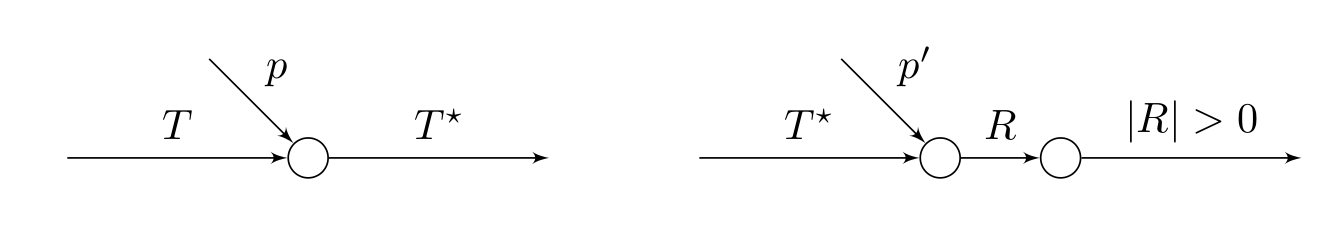
\includegraphics[width=.8\textwidth]{schematic}
\par}

\subsubsection*{ Step 2: Evaluation standards for computational serendipity}
\begin{quote} {\em Using Step 1, clearly state what standards you use to evaluate the serendipity of your
    system. }\end{quote}

With our definition in mind, we propose the following standards for
computational serendipity:

\begin{quote}
\begin{description}
\item[\emph{Prepared mind}] \emph{The system can be said to have a
  prepared mind, consisting of previous experiences, background
  knowledge, a store of unsolved problems, skills, expectations, and
  (optionally) a current focus or goal.}
\item[\emph{Serendipity trigger}] \emph{The serendipity trigger is at
  least partially the result of factors outside the system's control.
  These may include randomness or simple unexpected events.  The
  trigger should be determined independently from the end result.}
\item[\emph{Bridge}] \emph{The system uses reasoning techniques
  associated with serendipitous discovery -- e.g.  abduction, analogy,
  conceptual blending -- and/or social or otherwise externally enacted
  alternatives.}
\item[\emph{Result}] \emph{A novel result is obtained, which is
  evaluated as useful, by the system and/or by an external source.}
\end{description}
\end{quote}

\subsubsection*{Step 3: Testing our serendipitous system}

\begin{quote} {\em Test your serendipitous system against the standards stated in Step 2 and report the
results.}\end{quote}

In order to develop connections with our theoretical framework, and
because existing experiments have not been particularly strong, we
focus on a thought experiment in the following section, detailing some
of the outcomes we would like to see, and some of the risks.


\subsection{Related work} \label{sec:related}

An active research community investigating computational models of serendipity exists in the field of information retrieval, and specifically, in recommender systems \cite{Toms2000}. In this domain, \citeA{Herlocker2004} and \citeA{McNee2006} view serendipity as an important factor for user satisfaction, alongside accuracy and diversity.  Serendipity in recommendations variously require the system to deliver an \emph{unexpected} and \emph{useful}, \emph{interesting}, \emph{attractive} or \emph{relevant} item. 
% \cite{Herlocker2004} \cite{Lu2012},\cite{Ge2010}.  
Definitions differ as to the requirement of \emph{novelty}; \citeA{Adamopoulos2011}, for example, describe systems that suggest items that may already be known, but are still unexpected in the current context.  While standardized measures such as the $F_1$-score or the (R)MSE are used to determine the \emph{accuracy} of a recommendation (as very close to what the user is known to prefer), there is no common agreement on a measure for serendipity yet, although there are several proposals \cite{Murakami2008, Adamopoulos2011, McCay-Peet2011,iaquinta2010can}.
  In terms of our model, these systems focus mainly on producing a \emph{serendipity trigger} for the user and in support of discovery, but they include aspects of user modeling which could bring other elements into play, as we will discuss in Section \ref{sec:computational-serendipity}.

Recent work has examined related topics of \emph{curiosity}
\cite{wu2013curiosity} and \emph{surprise} \cite{grace2014using} in
computing.  This latter work seeks to ``adopt methods from the field
of computational creativity [$\ldots$] to the generation of scientific
hypotheses.''  In contrast to the typical application of recommender
systems, this is an example of an effort focused on computational
invention.

Paul Andr{\'e} et al.~\citeyear{andre2009discovery} have examined
serendipity from a design perspective.  Like us, these authors
proposed a two-part model encompassing ``the chance encountering of
information, and the sagacity to derive insight from the encounter.''
According to Andr\'e et al., the first phase is the one that has most
frequently been automated -- but they suggest that computational
systems should be developed that support both aspects.  They
specifically suggest to focus on representational features:
\emph{domain expertise} and a \emph{common language model}.

Although tremendously useful when they are available, these features
are not always enough to account for serendipitious events.  Using the
terminology we introduced earlier, these features seem to exemplify
aspects of the \emph{prepared mind}.  However, as we mentioned above,
the \emph{bridge} is a distinct process that mental preparation can
support, but that it does not necessarily fully determine.  For example, participants in
a poetry workshop may possess a very limited understanding of each
other's aims or of the work they are critiquing, and may as a
consequence talk past one another to a greater or lesser degree --
while nevertheless finding the overall process of participating in the
workshop itself illuminating and rewarding (often precisely because
such misunderstandings elucidate poor communication choices!).
Various social strategies, ranging from Writers Workshops to open
source software, pair programming, and design charettes
\cite[p. 11]{gabriel2002writer} have been developed to exploit similar
emergent effects and to develop \emph{new} shared language.  In
\cite{poetry-workshop}, we investigate the feasibility of using
designs of this sort in multi-agent systems that learn by sharing and
discussing partial understandings.  This earlier paper remains broadly
indicative, however, and the ideas it describes can see considerable
benefit from the more formal thinking we develop in the current work.

\citeA{robot-rendezvous} develop a discussion of serendipitous
rendezvous in a multi-agent system for a graph exploration problem, in
which ``[h]aving more data about their colleagues, better decisions
are made about the potential serendipity path.''  This has some
similarity to the discursive scenario described above, and shows that
\emph{asymmetric partial knowledge} can support serendipitious
findings.  These examples suggest that a distinction between emergent
knowledge of other actors and knowledge about an underlying domain may
be useful -- although the distinction may be less relevant if
the underlying domain itself has dynamic and emergent features.
\emph{Social coordination} among human users of information systems is
a current research topic. \citeA{rubin2010everyday} point out that
naive end users often \emph{talk about} serendiptious occurrences,
which presents another route for research and evaluation.

The {\sf SerenA} system developed by Deborah Maxwell et al.~\citeyear{maxwell2012designing} offers a case study of several of the points discussed above.
This system is designed to support serendipitous discovery for its (human) users
\cite{forth2013serena}.  The authors rely on a process-based model of
serendipity \cite{Makri2012,Makri2012a} that is derived from user
studies, including interviews with 28 researchers, looking for
instances of serendipity from both their personal and professional
lives.  This material was coded along three dimensions:
\emph{unexpectedness}, \emph{insightfulness}, and \emph{value}.  This
research aims to support the process of forming bridging connections
from unexpected encounter to a previously unanticipated but valuable
outcome.  The theory focuses on the acts of \emph{reflection}
that foment both the creation of a bridge and estimates of the
potential value of the result.
%
While this description touches on all of the features of our model, {\sf
  SerenA} largely matches the description offered by Andr{\'e} et
al.~\citeyear{andre2009discovery} of discovery-focused systems, in which
is user experiences an ``aha'' moment and takes the
creative steps to realise the result.  {\sf SerenA}'s primary computational method is to
search outside of the normal search parameters in order to engineer
potentially serendipitous (or at least pseudo-serendipitous)
encounters.
%% Another
%% earlier related example of this sort of system is {\sf Max}, created
%% by Figueiredo and Campos \citeyear{Campos2002}.  The user emailed {\sf
%%   Max} with an existing list of interests and {\sf Max} would return a
%% web page that might also be of interest.  Other systems with similar
%% support for serendipitous discovery involve searching for analogies
%% \cite{Donoghue2002,Donoghue2012}) as well as content \cite{Iaquinta2008}.

In recent joint work \cite{colton-assessingprogress}, we presented a
diagrammatic formalism for evaluating progress in computational
creativity.  It is useful to ask what serendipity would add to this
formalism, and how the result compares with other attempts to
formalise serendipity, notably Figueiredo and Campos's
\citeyear{Figueiredo2001} `Serendipity Equations'.  In this work,
Figueiredo and Campos describe serendipitous ``moves'' from one
problem to another, which transform a problem that cannot be solved
into one that can.  In our diagrammatic formalism, we spoke about
progress with \emph{systems} rather than with \emph{problems}.  It
would be a useful generalisation of the formalism -- and not just a
simple relabelling -- for it to be able to tackle problems as well.
However, it is important to notice that progress with problems does not always mean transforming a
problem that cannot be solved into one that can.  Progress may also
apply to growth in the ability to \emph{posit} problems.  In keeping
track of progress, it would be useful for system designers to record
(or get their systems to record) what problem a given system solves,
and the degree to which the computer was responsible for coming up
with this problem.

As \cite[p. 69]{pease2013discussion} remark, anomaly detection and
outlier analysis are part of the standard machine learning toolkit --
but recognising \emph{new} patterns and defining \emph{new} problems
is more ambitious.  Complex analogies between evolving problems and
solutions form one of the key strategies for teams of human designers
\cite{Analogical-problem-evolution-DCC}.  Kazjon Grace
\citeyear{kaz-thesis} presents one computational model of the creation
of new concepts and interpretations, but this work did include the
ability to create new higher order relationships necessary for complex
analogies.  New patterns and higher-order analogies were considered in
Hofstadter and Mitchell's {\sf Copycat} and the subsequent {\sf
  Metacat}, but these systems operated in a simple and fairly abstract
``microdomain''
\cite{hofstadter1994copycat,DBLP:journals/jetai/Marshall06}.  %% More
%% recent work in this tradition is surveyed in
%% \cite{eric-nichols-thesis}.

The relationship between serendipity and novel problems receives
considerable attention in the current work, since we want to
increasingly turn over responsibility for creating and maintaining a
prepared mind to the machine.

